\documentclass{article}
\usepackage[margin=1in]{geometry}
\usepackage{hyperref}
\usepackage{pdfpages}

\title{Absorption Spectroscopy of Sodium through Magnetic Resonant Pulsing:\\
Notes}
\author{Adam Newton Wright}
\begin{document}

\maketitle

\begin{abstract}
  This documents aim to provide all the resources and notes that I may need for my senior thesis. The first section is my Senior Proposal, as part of an ATEP project. I then include all of the resources that I have used thus far, along with notes for each resource.
\end{abstract}

\pagebreak
\tableofcontents


\pagebreak

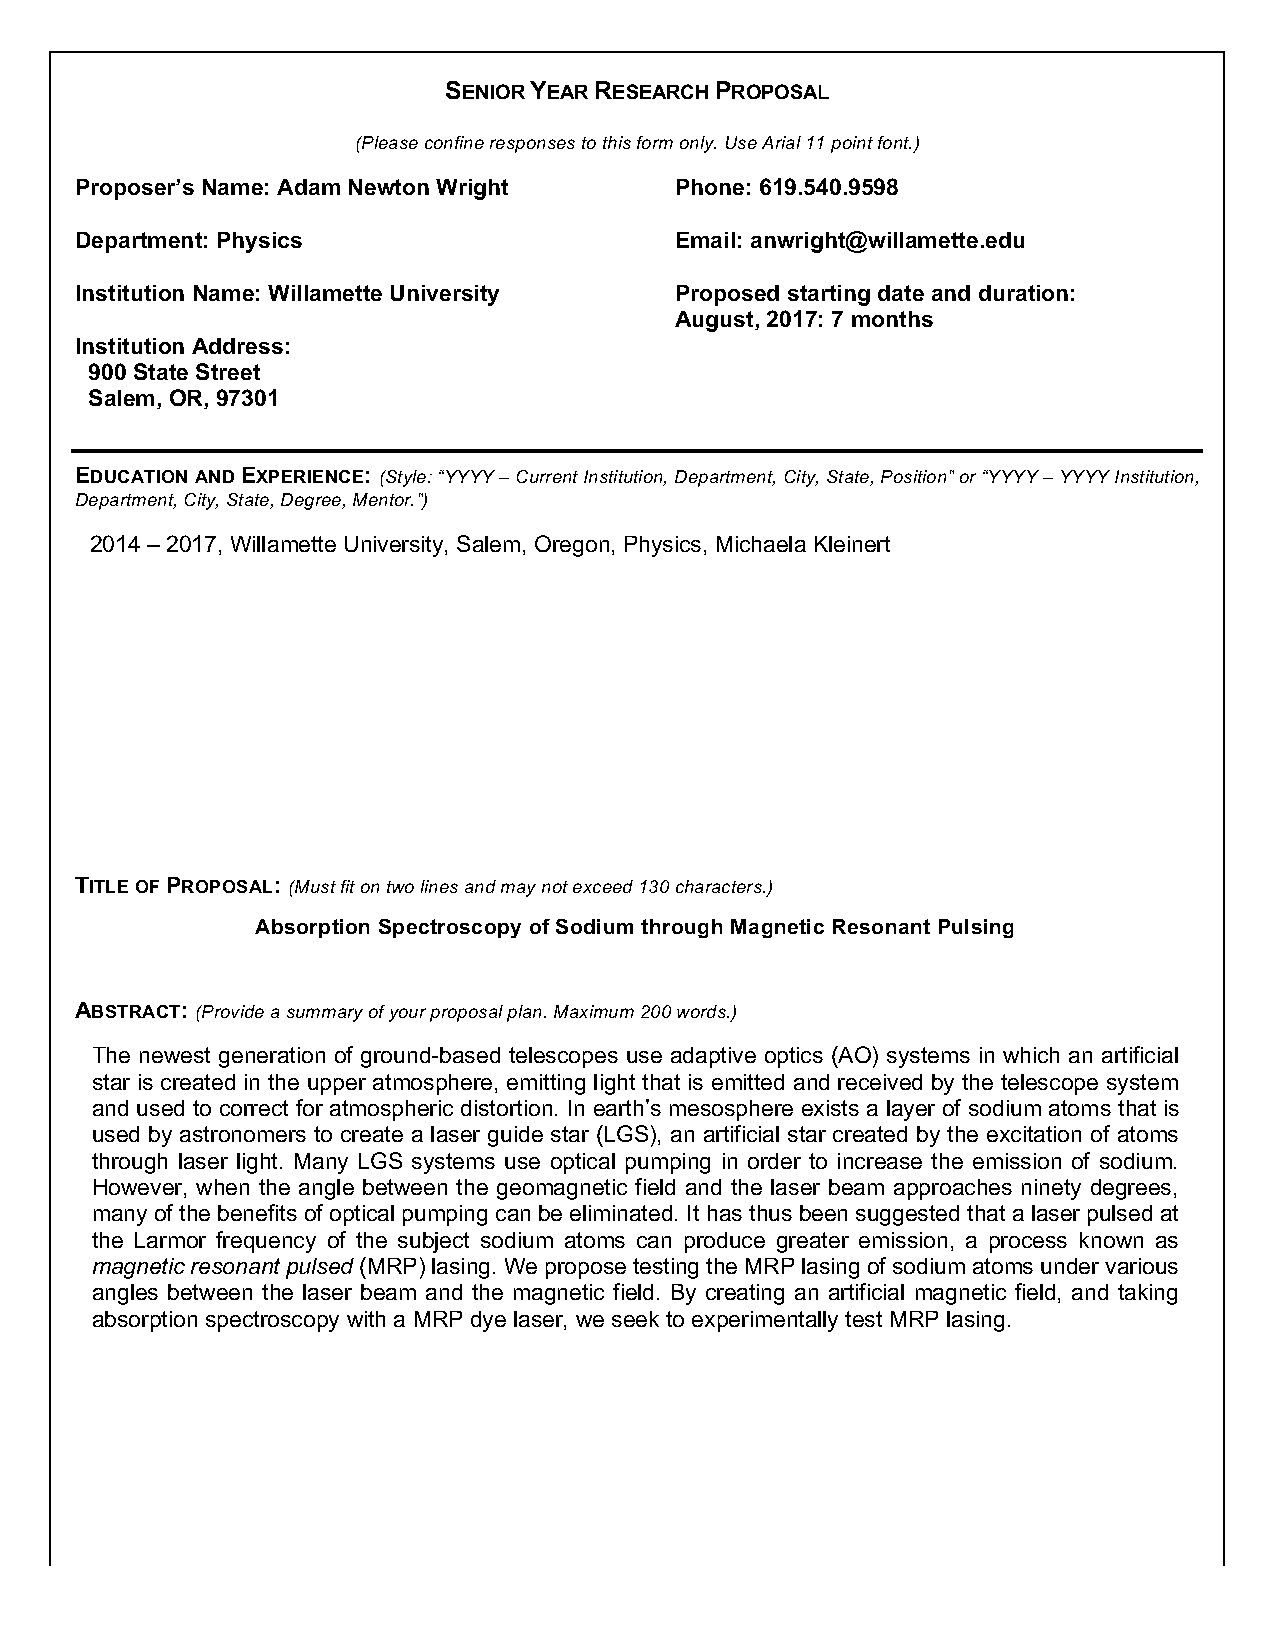
\includepdf[pages = -]{PDF/senior_proposal.pdf}
\pagebreak
\section{Senior Proposal}
\subsection{Abstract}
The newest generation of ground-based telescopes use adaptive optics (AO) systems in which an artificial star is created in the upper atmosphere, emitting light that is emitted and received by the telescope system and used to correct for atmospheric distortion. In earth’s mesosphere exists a layer of sodium atoms that is used by astronomers to create a laser guide star (LGS), an artificial star created by the excitation of atoms through laser light. Many LGS systems use optical pumping in order to increase the emission of sodium. However, when the angle between the geomagnetic field and the laser beam approaches ninety degrees, many of the benefits of optical pumping can be eliminated. It has thus been suggested that a laser pulsed at the Larmor frequency of the subject sodium atoms can produce greater emission, a process known as magnetic resonant pulsed (MRP) lasing. We propose testing the MRP lasing of sodium atoms under various angles between the laser beam and the magnetic field. By creating an artificial magnetic field, and taking absorption spectroscopy with a MRP dye laser, we seek to experimentally test MRP lasing.


\subsection{Statement of Problem and Significance of Research}
\underline{Fundamental Scientific Problem}\\
LGS are artificial star images created for usage in adaptive optics (AO) systems in order to increase the resolution of ground-based telescope imaging. Sodium LGSs are produced by sending laser into the upper atmosphere at the resonant frequency of sodium; this laser light excites a layer of sodium that exists in the mesosphere (Rampy 2015), and is then emitted by these sodium atoms, creating a visible “star.” The light from this LGS is then collected by a ground telescope and fed into an AO system where it is used to correct for atmospheric distortions that occur as light enters earth’s atmosphere (Fugate, Wizinowich 2009). The AO system corrects for these distortions by measuring the amount of distortion that the LGS light undergoes, and adjusts a deformable mirror to correct for these distortions. It can then use these corrections to collect higher resolution images.\\
LGSs needs to be sufficiently bright in order for the AO system to collect enough light to correct for distortions (Watanabe 2004). Typical LGS lasers operate at an intensity of  (Kane 2014) and can be CW or pulsed. The LGS lasers are circularly polarized, which allows the atom, after being excited and emitting a photon, to move to an angular momentum state with increased probability of backscattering; this creates a pumping cycle which in beneficial for greater emission, a process known as optical pumping (Fan, Kane 2014). The fundamental problem, however, is that the benefits of optical pumping can be almost completely eliminated when the angle between the laser light and the magnetic field approaches ninety degrees (Kane 2014); this is due to the fact that the magnetic field reorients the atom before it can properly redistribute its angular momentum.\\
\underline{Significance of the Problem}\\
Unfortunately, the majority of ground-based telescopes are relatively close to the equator, which corresponds to an angle close to ninety degrees when the laser is sent into the atmosphere. This in turn results in decreased emission of sodium atoms in the atmosphere, and a decreased efficiency of the LGS system. In order for AO systems to properly correct for atmospheric distortions, and in turn create higher resolution images, the LGS used must be sufficiently bright. By finding a way to reduce the negative effects of optical pumping at angles of ninety degrees between pump beam and the magnetic field, AO systems can not only function better, but will be much more efficient.\\
\underline{Originality of Approach}\\
It has been suggested that by pulsing the LGS laser at the Larmor frequency of the sodium atom in what is called MRP results in greater emission of sodium at all angles between the laser light and the magnetic field. Sodium has a magnetic moment, and thus, when within a magnetic field, will precess about its magnet moment, in a process called Larmor precession (Rampy 2015). The frequency at which it precesses is known as the Larmor frequency. Furthermore, the Larmor frequency is equal to the energy between the states split by the Zeeman structure; thus, the Larmor frequency corresponds to the inverse of the lifetime an electron is in an excited Zeeman state. Hence, by pumping sodium at this frequency, as soon as an atom has absorbed and emitted a photon, it is excited by another photon, allowing it to stay in its angular momentum state and continue its pump cycle.\\
Kane et al. used simulation software developed by Rochester Scientific to test MRP lasing. His data show that MRP lasing creates greater emission of sodium for all angles between the magnetic field and the laser light. I in turn propose testing this in the laboratory. By studying these processes in the laboratory, I intend to understand better how light interacts with atoms within a magnetic field and how their Larmor precession plays a role in their absorption and emission of light. Furthermore, understanding these ideas more clearly has direct implications to improving the efficiency and functionality of LGS systems.\\
To the best of our knowledge, this will be the first experimental testing of the MRP lasing of sodium. This is thus novel not only in regards to understanding how light pulses interact with atoms under the Zeeman structure, but also to creating a more efficient and functional LGS systems.\\
\underline{Hypothesis}
In this project I aim to show that the magnetic resonant pulsing (MRP) of sodium within a magnetic field produces greater emission for all angles between the magnetic field and the laser beam than pulsing at a frequency not equal to the magnetic resonant frequency.\\



\subsection{Plan of Procedure}
Month 1: We first need to test the feasibility of a MRP dye laser. The Larmor frequency of sodium is given by  where B is the magnetic field and  is the gyromagnetic ration given by  with e being the electric charge, g being the g-factor, and m being the mass of the atom. For a sodium atom on earth, this corresponds to a frequency of . During this first month, we will work on creating a tunable, pulsed dye laser (Sohl, 1997). This dye laser will consist of a dye cell filled will Rhodamine 610, which will enable the laser to emit light around the necessary 589.6 nm (Brackman 2000). Its cavity will consist of two mirrors and a diffraction grating, allowing us to select the corresponding wavelength of light.\\
Month 2: We need to configure our pump laser so that it will be able to pulse with the corresponding Larmor frequency and have a pulse width in the nanosecond regime; this can be accomplished by using a Duetto Nd:YAG laser. This laser is capable of pulsing on the order of kHz, sufficient for the sodium contained in our magnetic field. However, certain modification will need to be made to obtain this pulse frequency. Furthermore, the Duetto currently outputs 1064 nm laser light; 532 nm light is necessary in order to properly excite the Rhodamine dye and obtain the proper wavelength of light to excite sodium at its 589 nm peak line. We thus need to purchase and configure a second harmonic generation crystal on the Duetto in order to frequency double the light. A KTP crystal can be bought from EKSMA Optics and configured to the laser quite easily.\\
Month 3: We will next begin configuring our previously constructed dye laser with our MRP Duetto pump laser. The feasibility of this is described by Gale (Gale 1990), but we expect certain difficulties to arise. These difficulties may include the dye not being circulated quick enough, poor beam profile, or poor lasing (Gale 2012).\\
Month 4: If the previous projects are successful, we will continue with this project and construct a more advanced configuration. We will first use a dye laser capable of producing a cleaner and amplified beam. The dye laser is a Continuum ND6K, with dual amplification cells. This dye laser can be configured and tuned according to the Continuum ND6K User Manual (Continuum). It will also need to be made compatible with the MRP Duetto laser, an aspect which has not been tested on this dye system before.\\
Month 5: The dye laser output beam will need to be characterized with respect to wavelength, linewidth, and bandwidth in order to ensure it can properly excite sodium. It will also need to be able to produce an intensity of . Furthermore, the dye laser output beam will need to be circularly polarized (Kane 2012), which requires nothing more than a few quarter wave plates.\\

Month 6: Once the dye laser is properly established, the sodium reference cell and measurement system will need to be constructed. The reference cell will be a borosilicate glass reference cells available from Thorlabs. This ensures that maximum green light is transmitted, about 80$\%$, and that the cell can withstand a temperature of 100 C, necessary to melt sodium. This cell will be mounted and wrapped in heating tape and filled with a small amount of Sodium. Lastly, a photodiode will be placed perpendicular to the length of the reference cell in order to collect transmitted light. We also will create a magnetic field around the reference cell. This can be done by created Helmholtz coils. We expect to create a magnetic field of , which corresponds to a current of approximately . We are able to 3D print a coil mount, and wrap this mount in wire and wire it to a power supply, which will need to be bought. The Helmholtz coils will need to be able to rotate around the reference cell, changing the angle between the magnetic field and the laser light.
Month 7: Data will finally be collected The laser light from the dye cell will be directed into the reference frame containing the sodium. The tunability of the dye laser is important, as we will measure the intensity of the light transmitted as a function of varying wavelength. At wavelengths close to 589 nm, the intensity of light should greatly decrease as sodium in absorbing this light and releasing it randomly. We then leave the dye laser at this wavelength and measure the intensity of transmitted light as the angle between the magnetic field and the dye beam is varied. We will then change the Duetto so that its pulse frequency is not at the Larmor frequency and repeat this process.
	 




\pagebreak

\section{Resources}
\subsection{Optical Magnetometry-Budker}
This paper details optical magnetometry. This related to the the absorbtion spectroscopy of sodium, which will be done later in the project.
\pagebreak

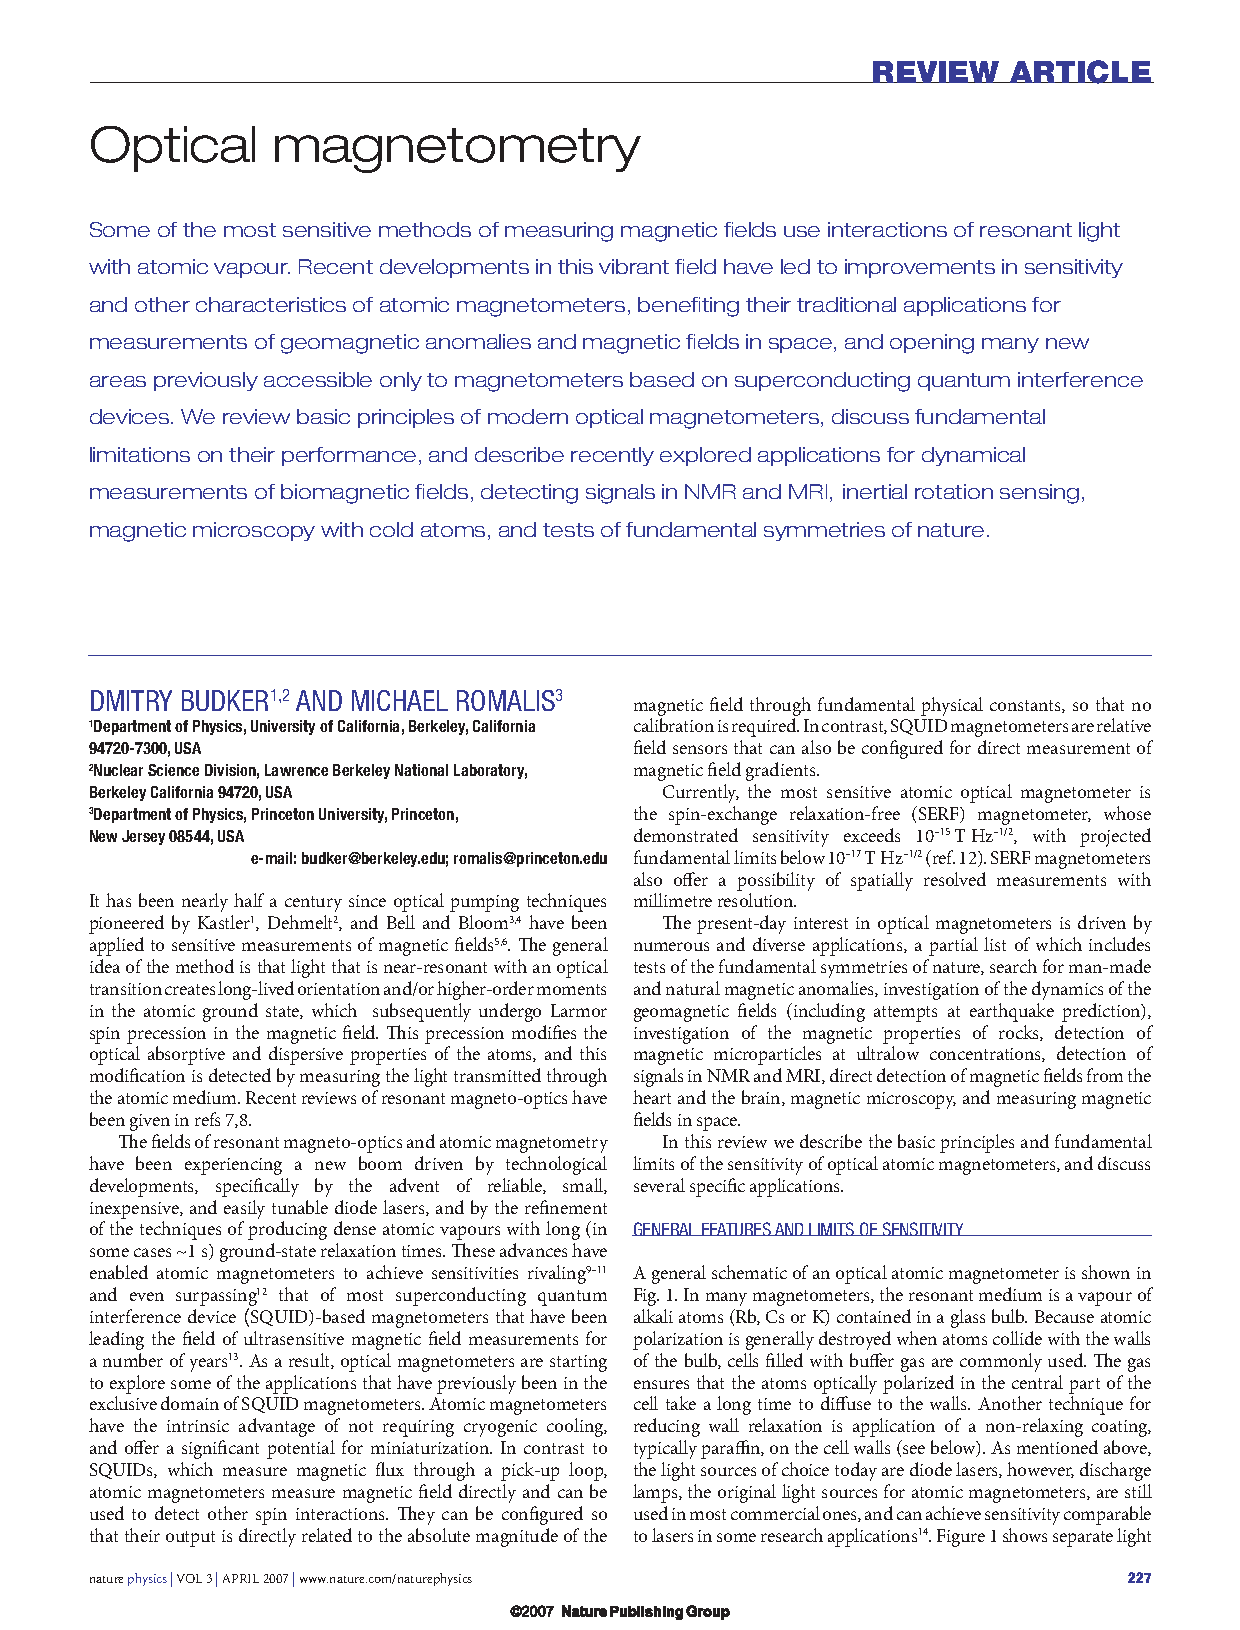
\includepdf[pages =-]{PDF/Optical_magnetometry.pdf}

\pagebreak

\subsection{Improving LGS through polarization switching - Fan}

\pagebreak
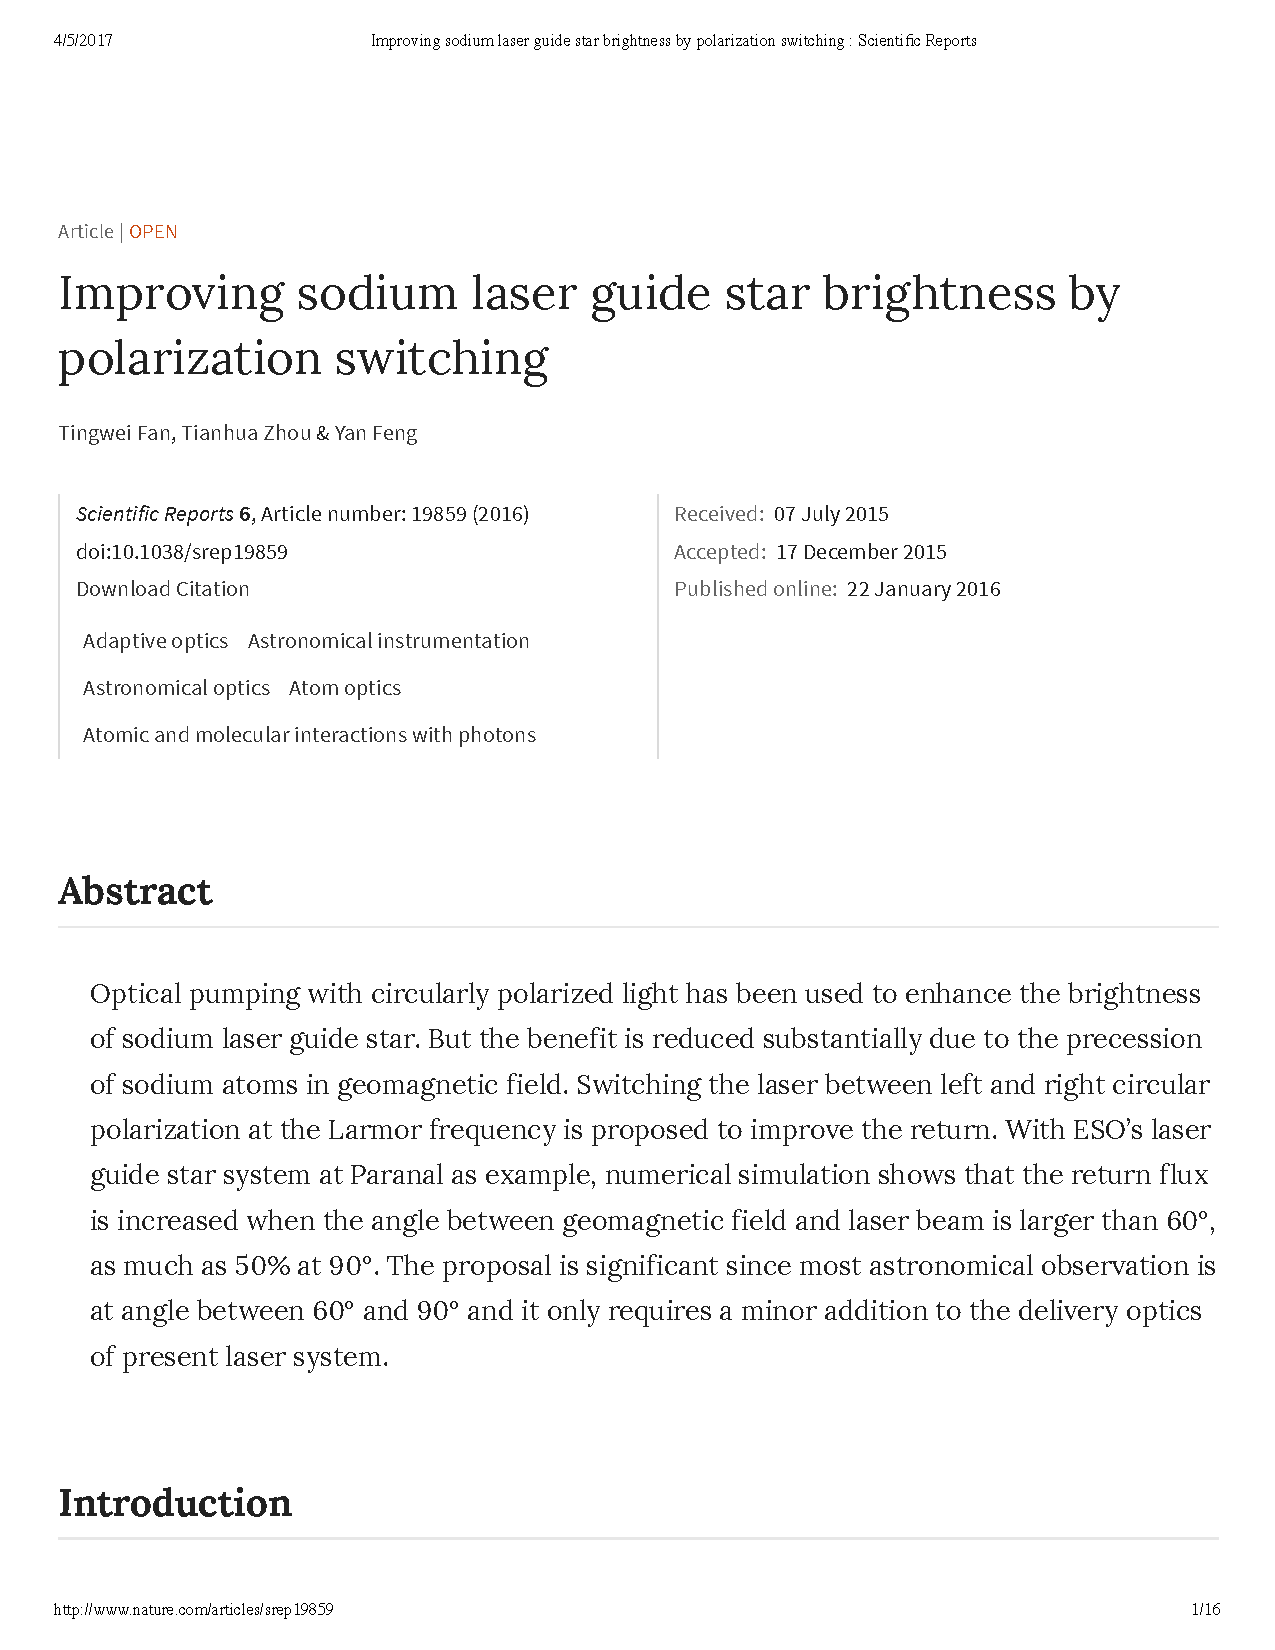
\includepdf[pages=-]{PDF/Improving_lgs_brightness_polarization_switching}
\pagebreak

\subsection{Improve Atmospheric Distortion Measurement - Fugate}
\pagebreak

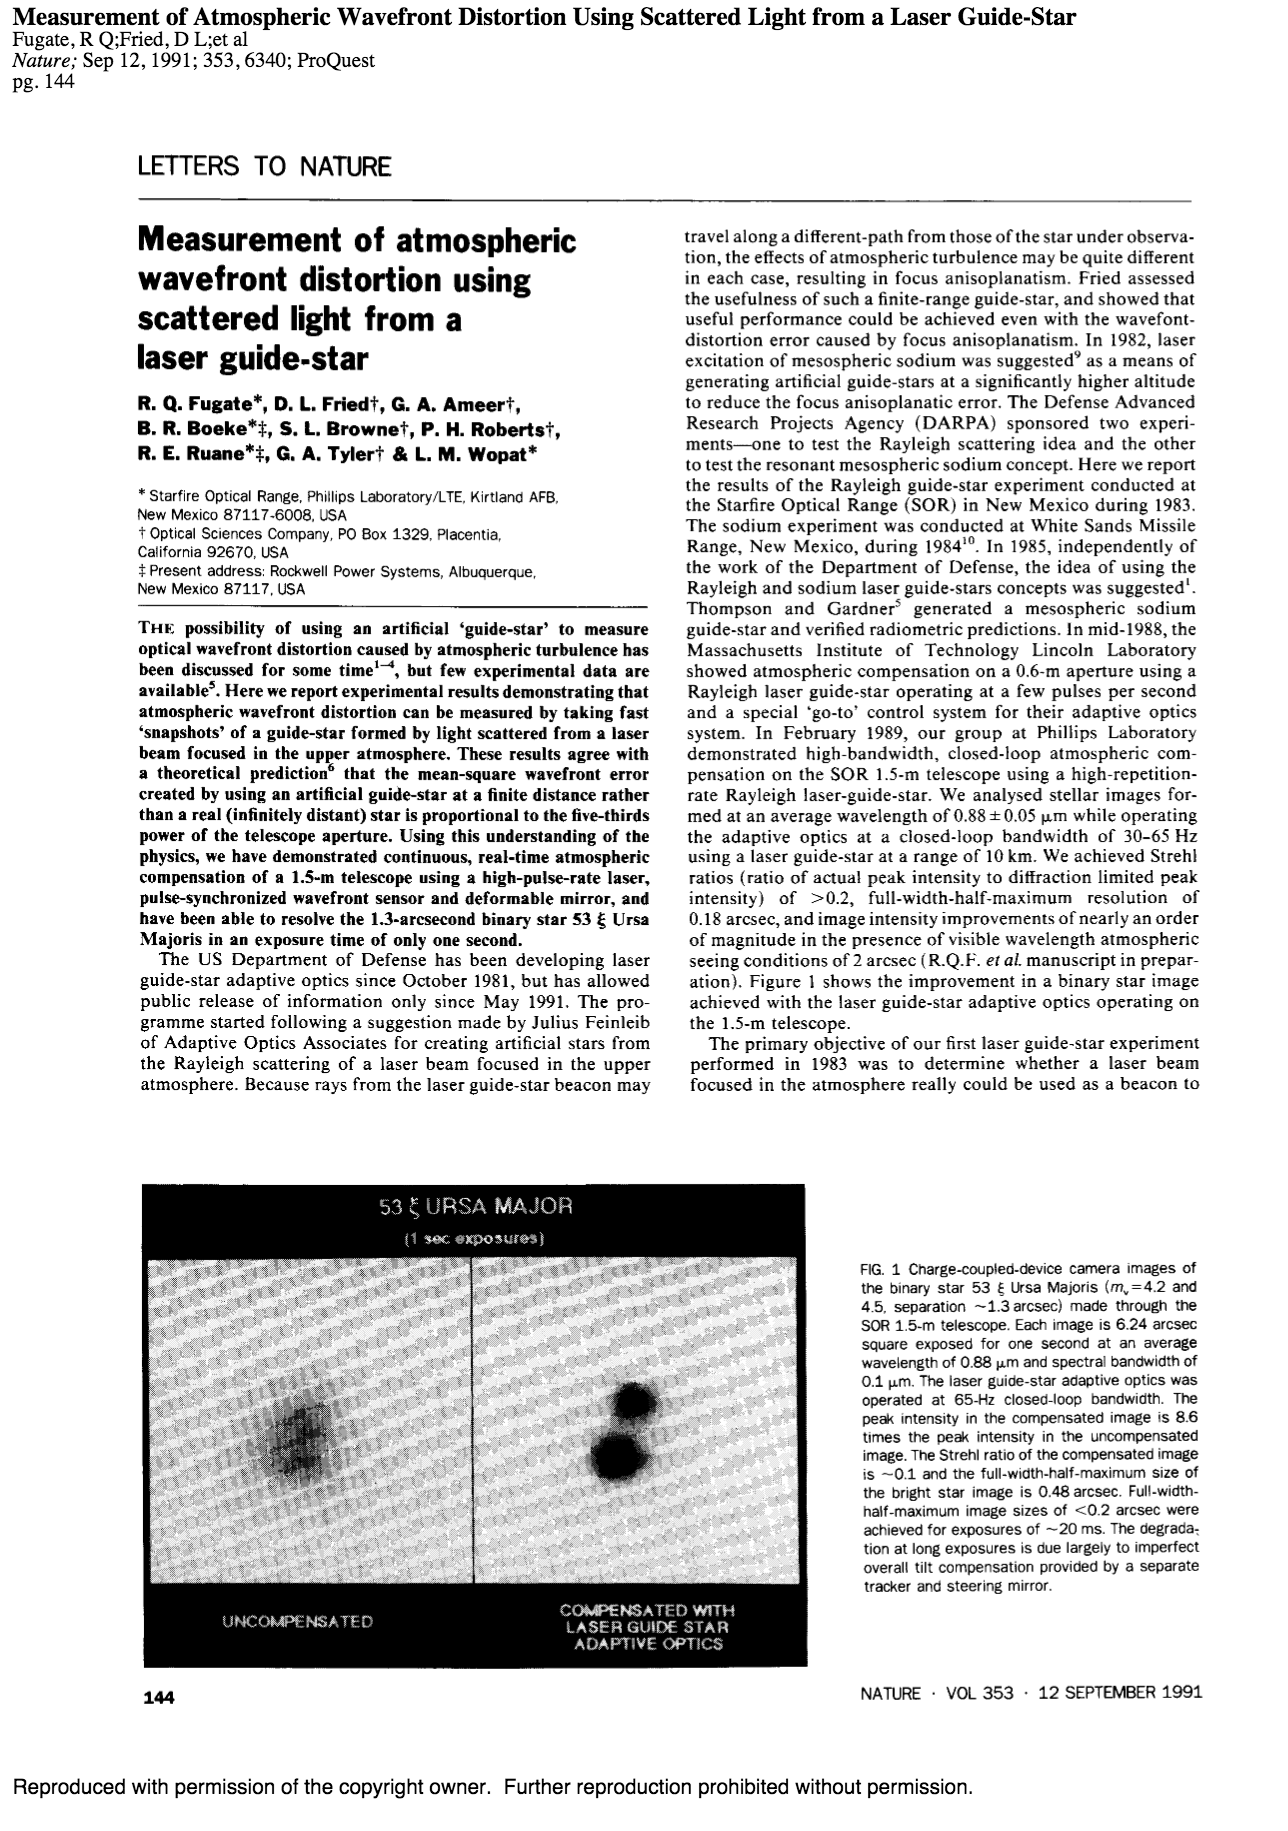
\includepdf[pages=-]{PDF/measurement_atmospheric_distortion.pdf}
\pagebreak

\subsection{Kilohertz Picosecond Dye Laser - Gale}
A light paper on a kilohertz picosecond dye laser.

\pagebreak
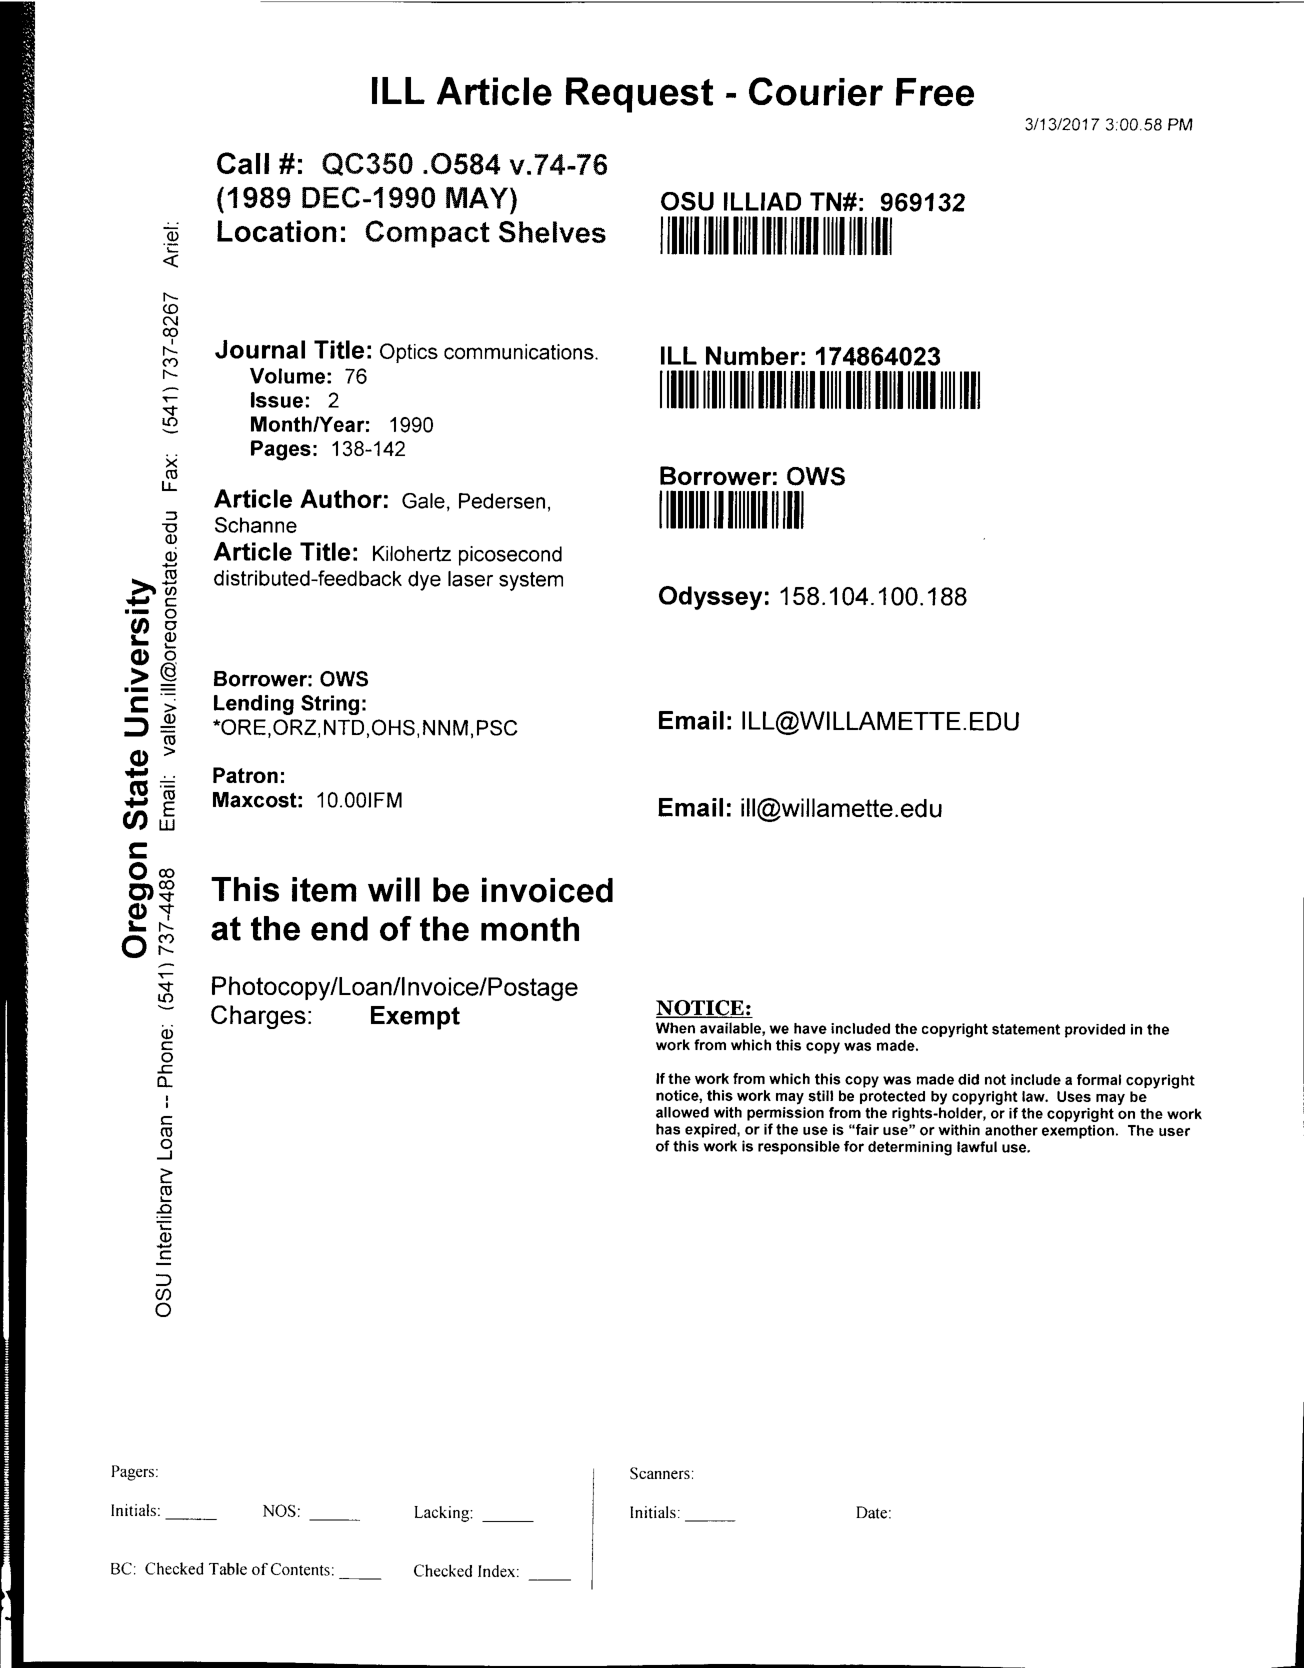
\includepdf[pages=-]{PDF/kilohertz_picosecond_dyelaser.pdf}
\pagebreak

\subsection{Magnetic Resonant Pulsing-Kane}
This first paper I believe is the most important paper to this project. It details magnetic resonant pulsing, and provides a lot of the background and theory behind the process.

\pagebreak

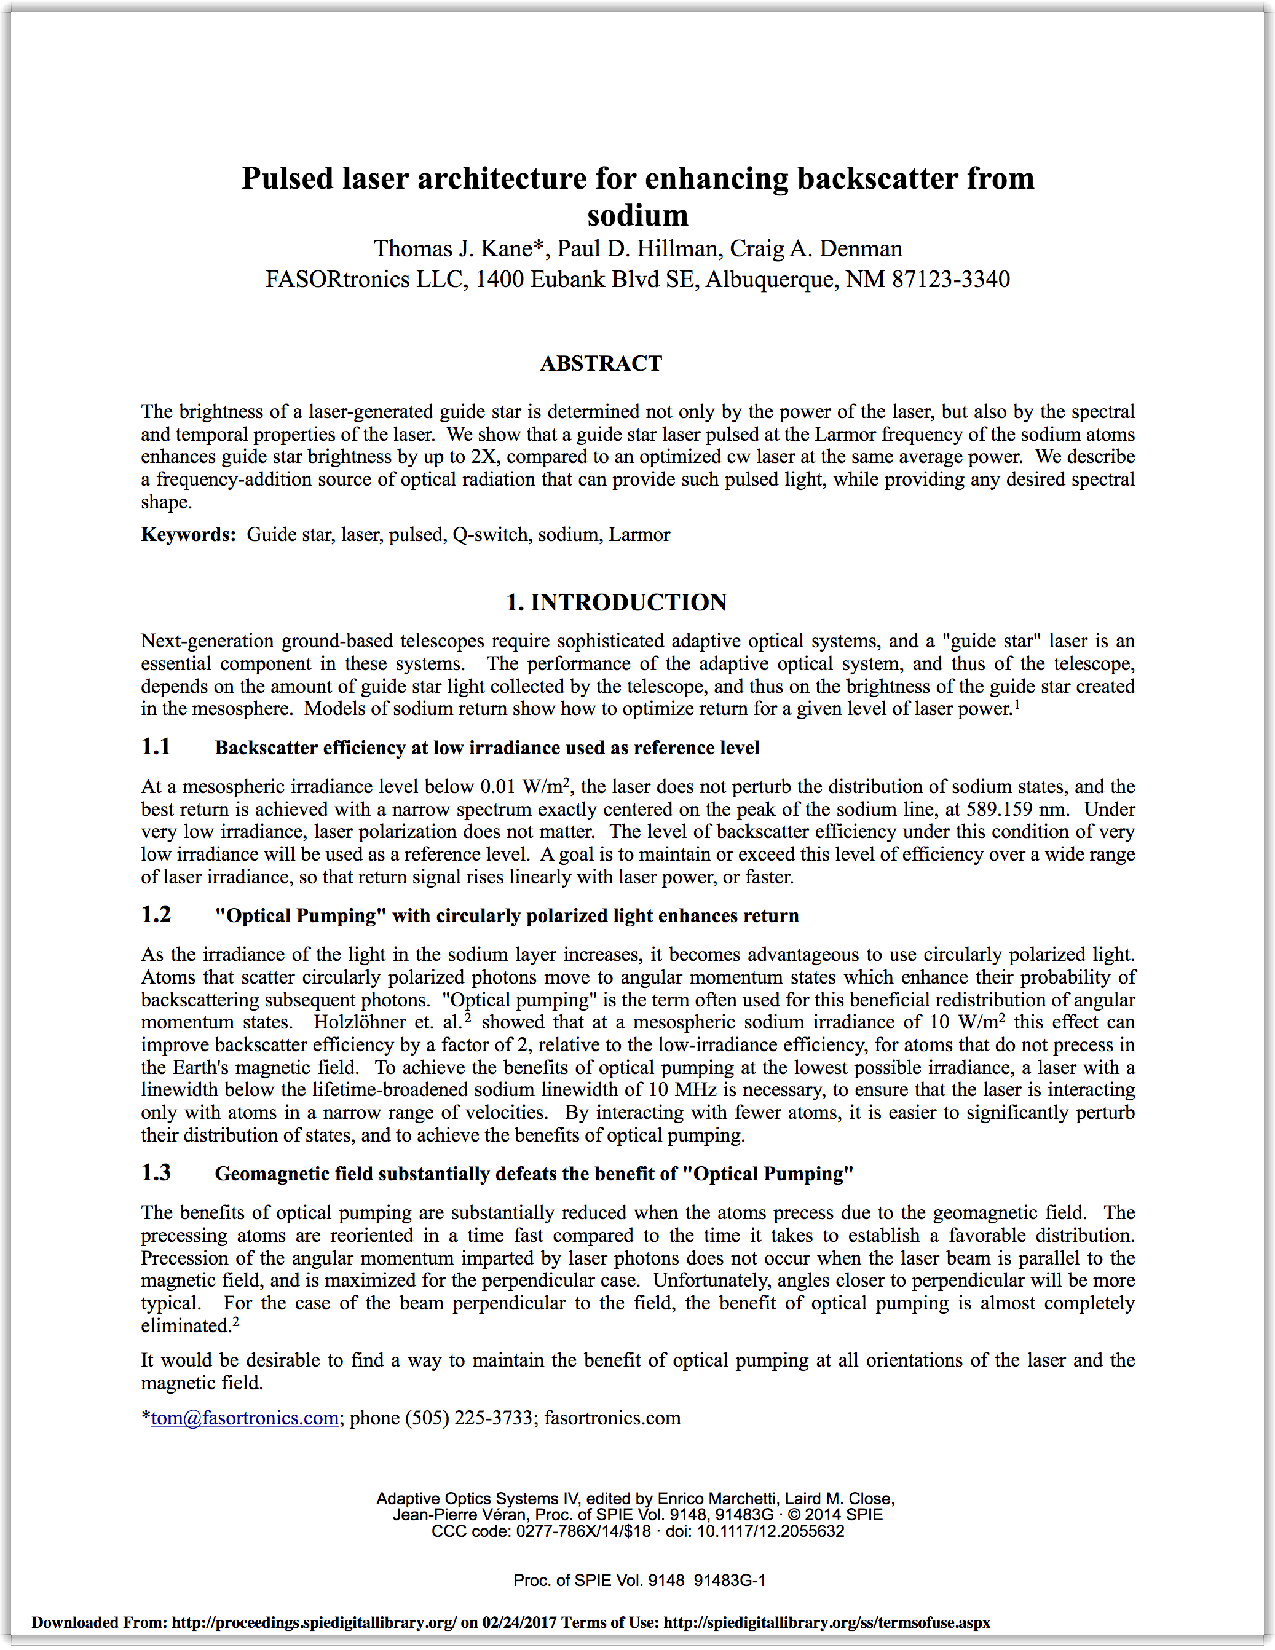
\includepdf[pages=-]{PDF/Pulsed_laser_architecture.pdf}

\pagebreak

\subsection{Physics of Sodium LGS - Kibblewhite}
You should read this paper more! Details the physics of LGS, and enters into quantum theory.

\pagebreak
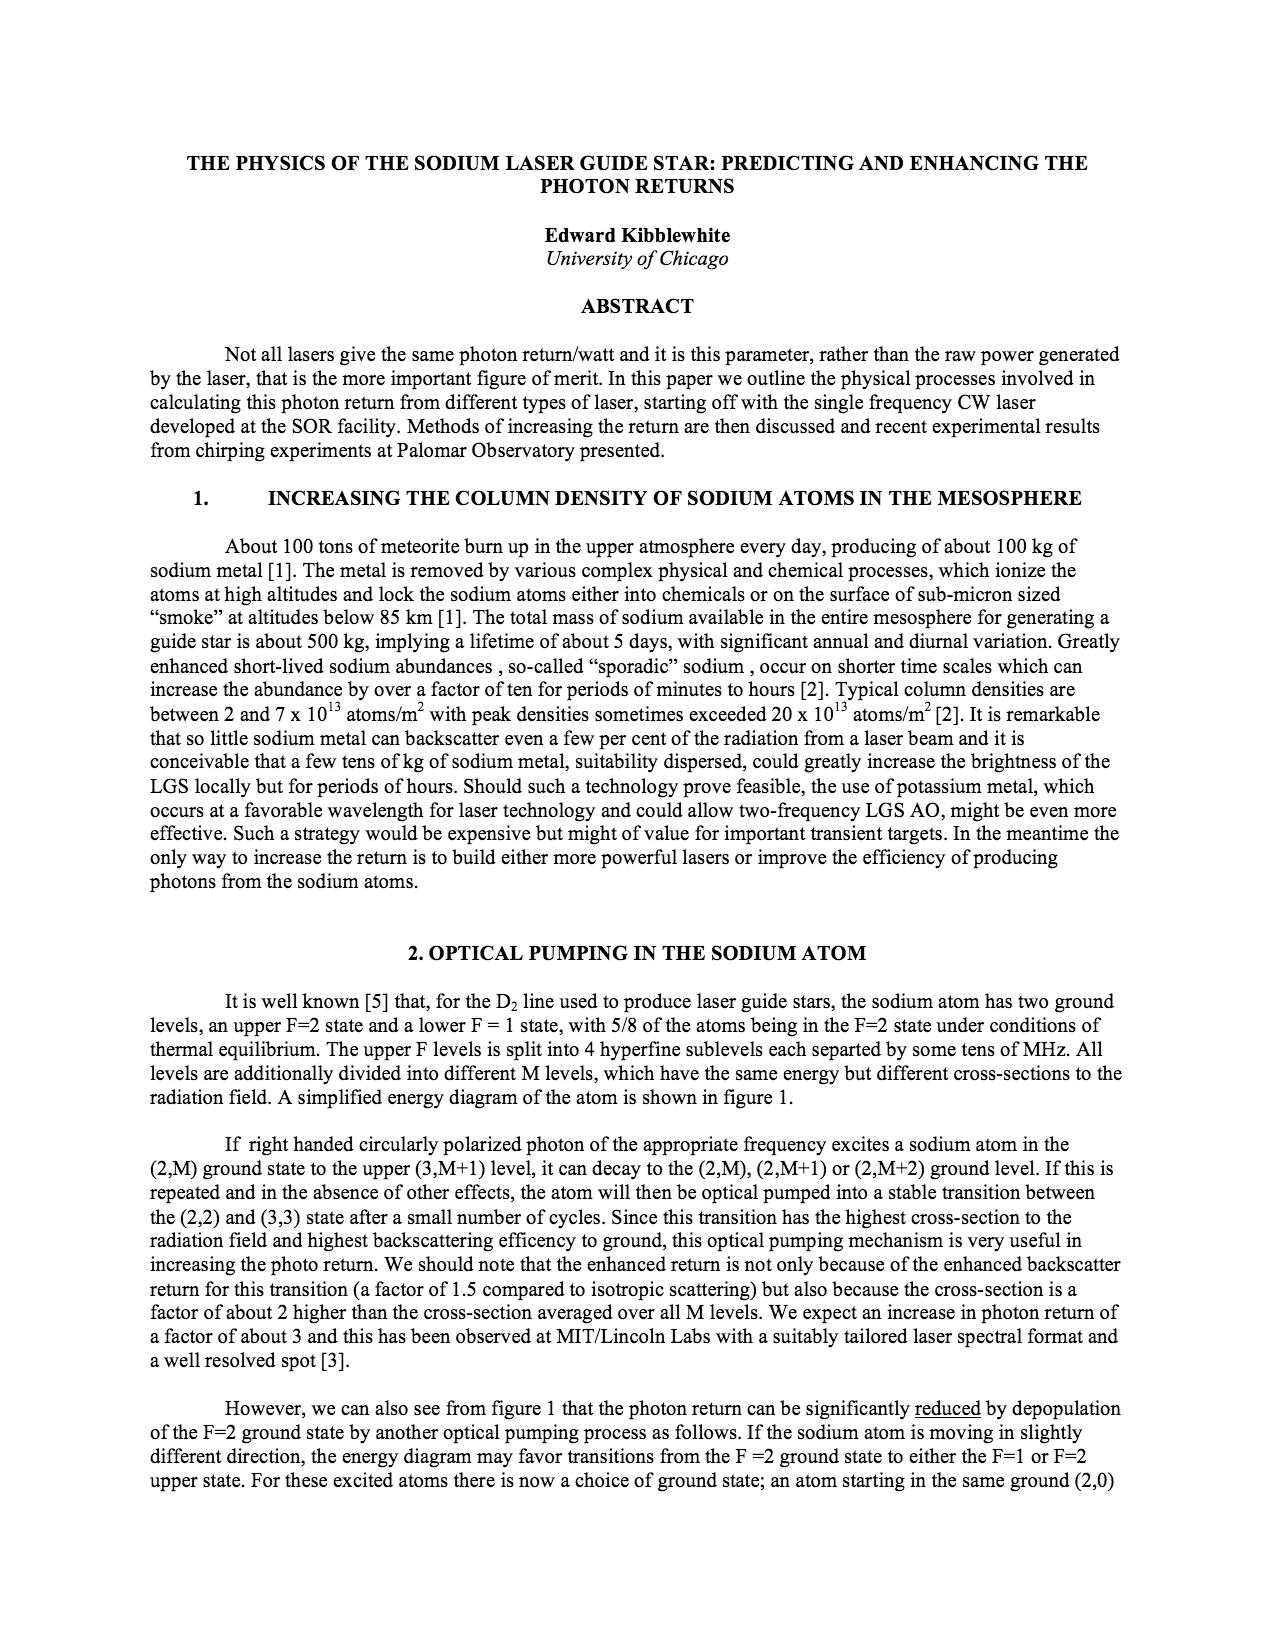
\includepdf[pages = 1]{PDF/physics_of_sodium_lgs.pdf}
\pagebreak

\subsection{Optimization of Pulsed LGS - Rampy}
This is the paper where I learned about larmor precession. Lightly touches on MRP as a solution.
\pagebreak
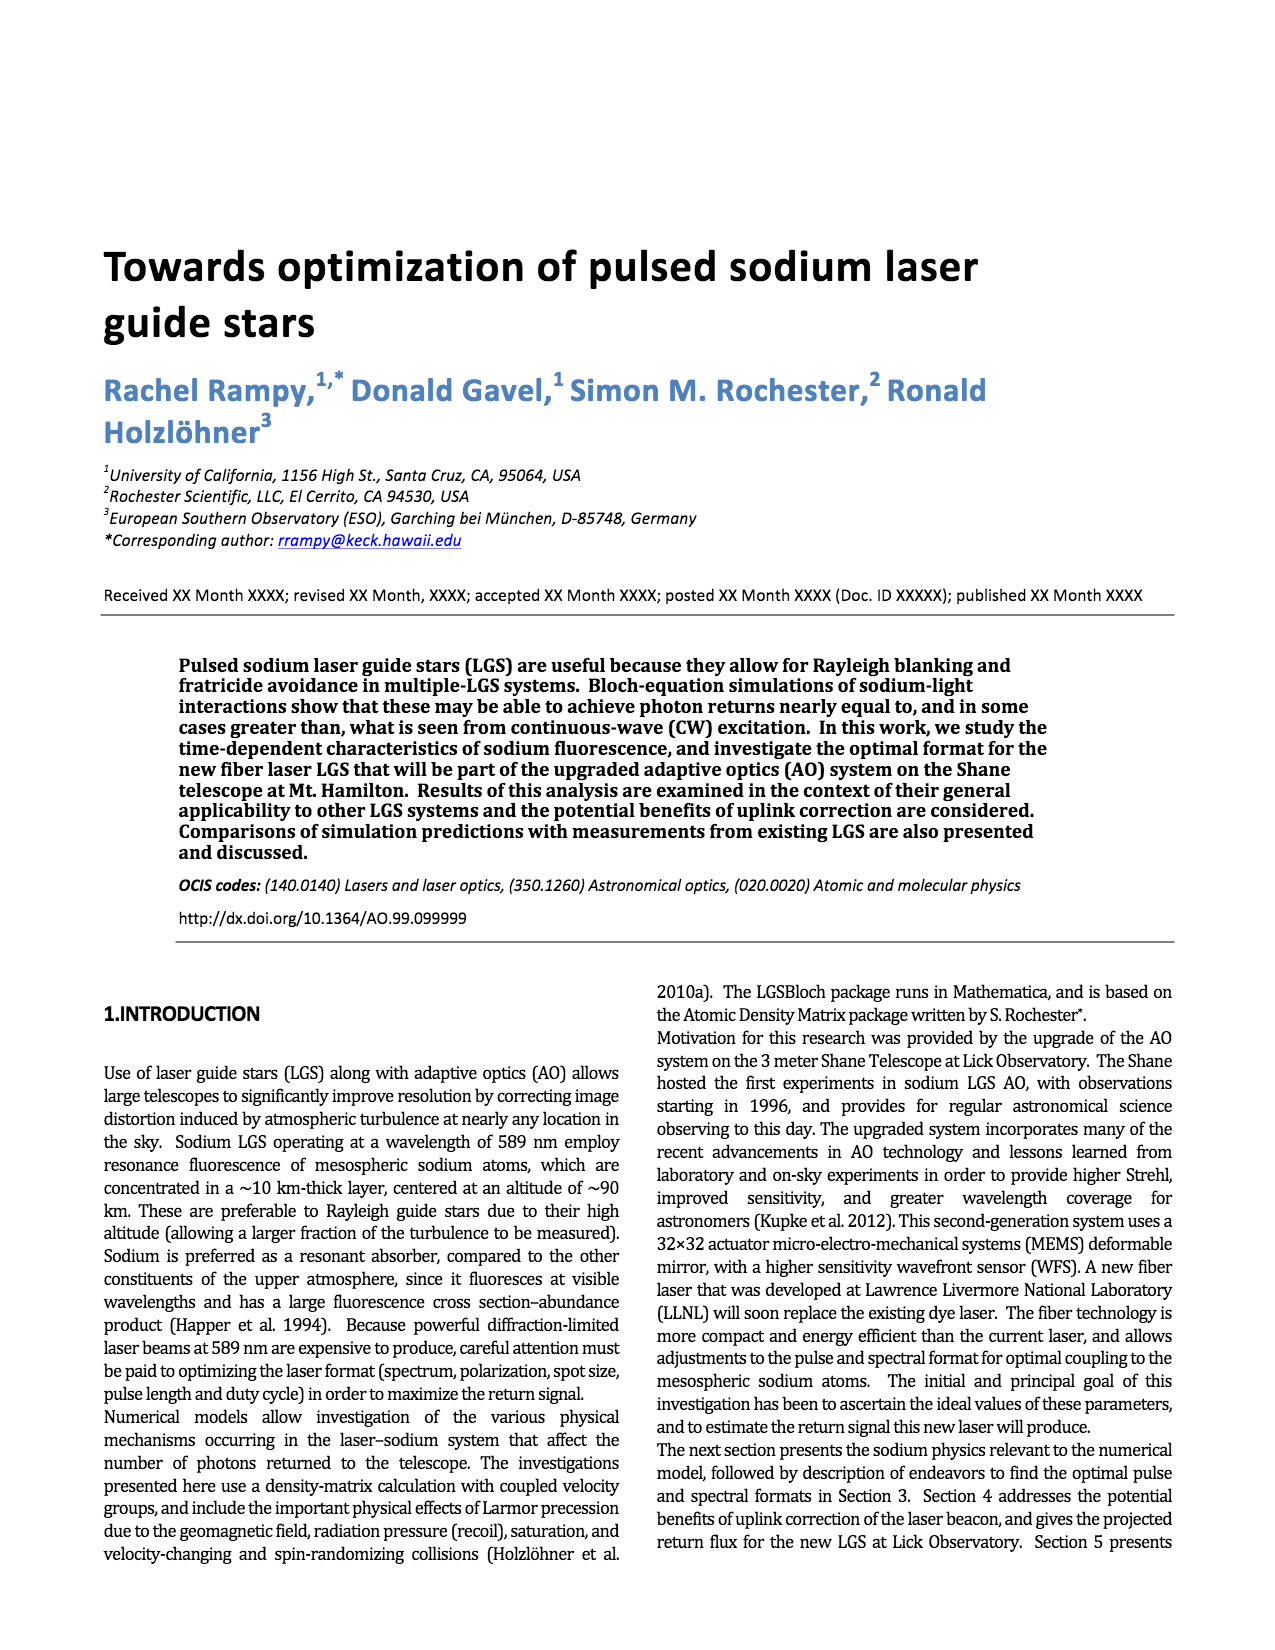
\includepdf[pages = -]{PDF/optimization_pulsed_lgs.pdf}
\pagebreak

\subsection{Optimization of CW LGS - Holzlohner (Rampy)}
I believe that this is a more in depth paper of the one above. I have not read it yet.
\pagebreak

\includepdf[pages=-]{PDF/optimization_of_cw_lgs.pdf}
\pagebreak

\subsection{Modular Reconfigurable Dye Laser of Undergrad Lab - AJP}
A nice text detailing how to set up a simple dye laser
\pagebreak
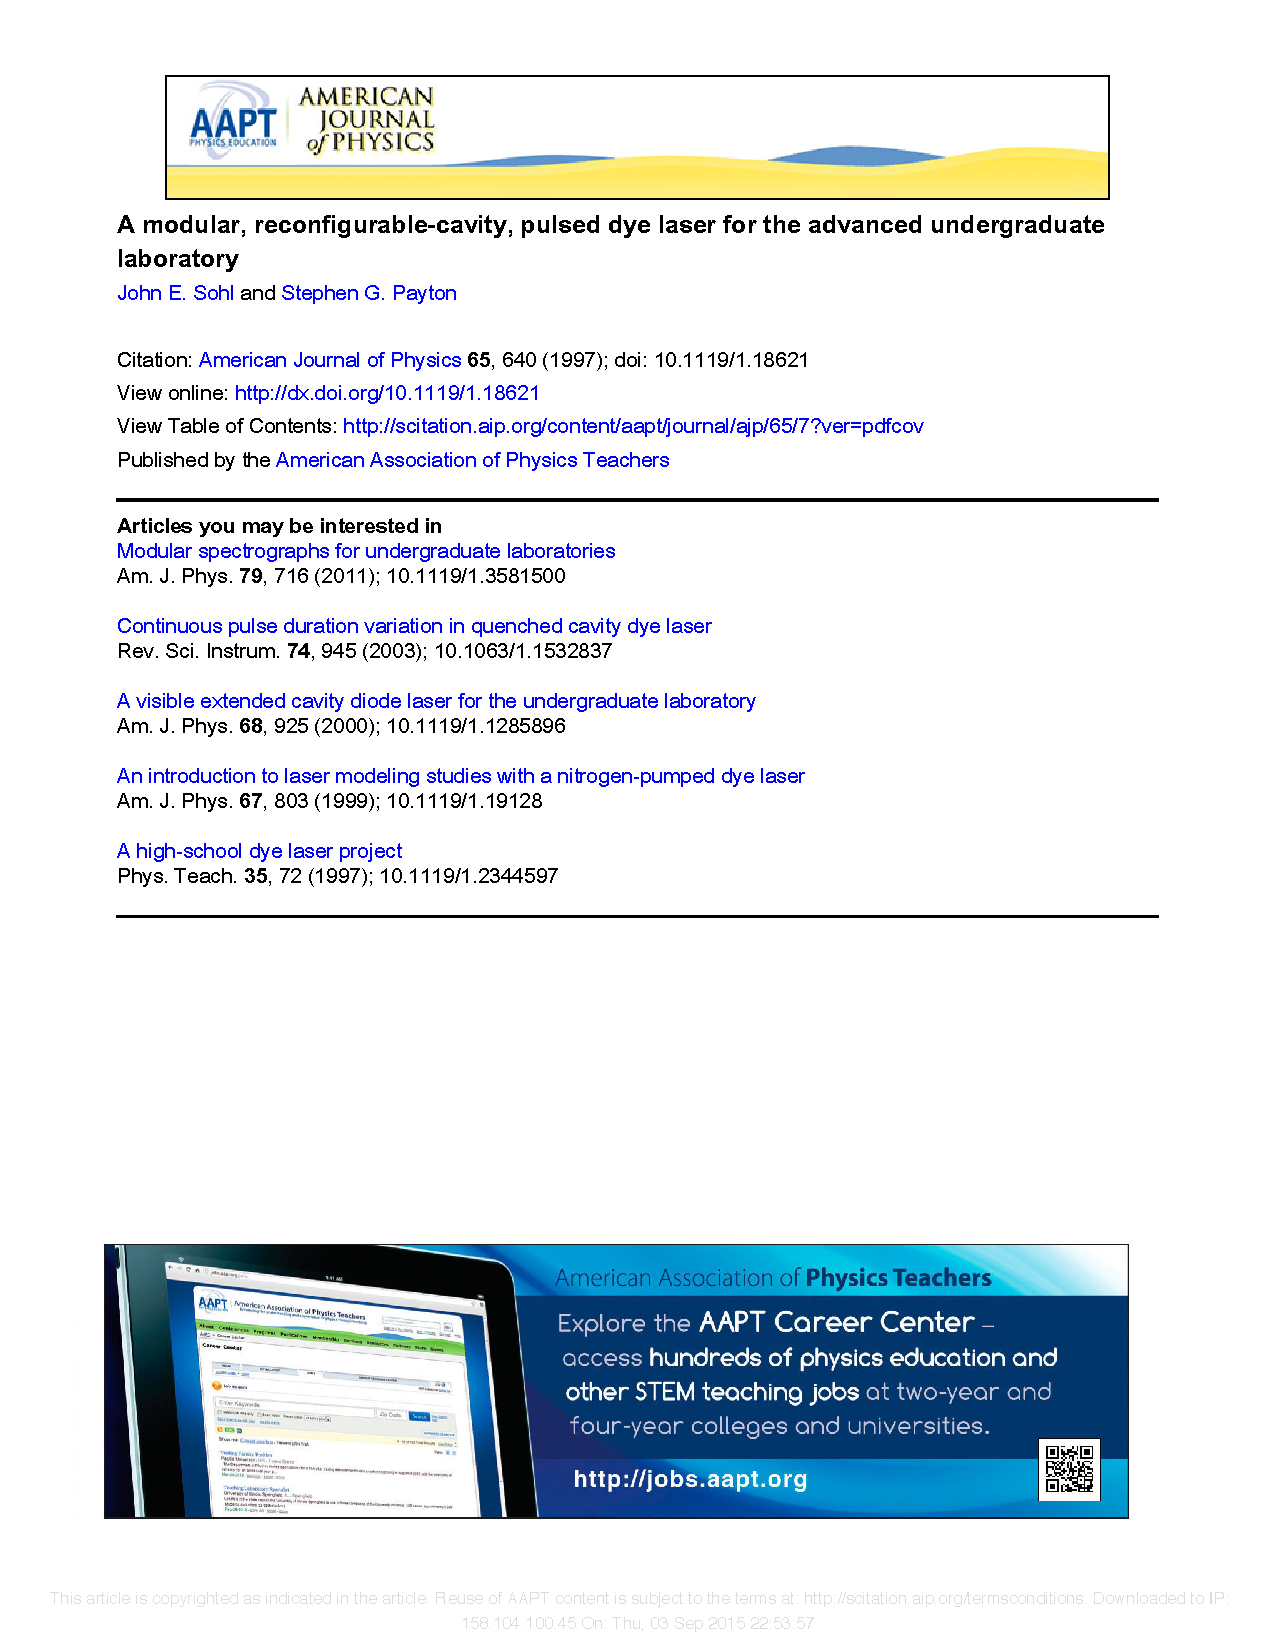
\includepdf[pages = -]{PDF/DyeLaserAJP.pdf}

\pagebreak
\subsection{W.M. Keck Observatory AO System}

\pagebreak
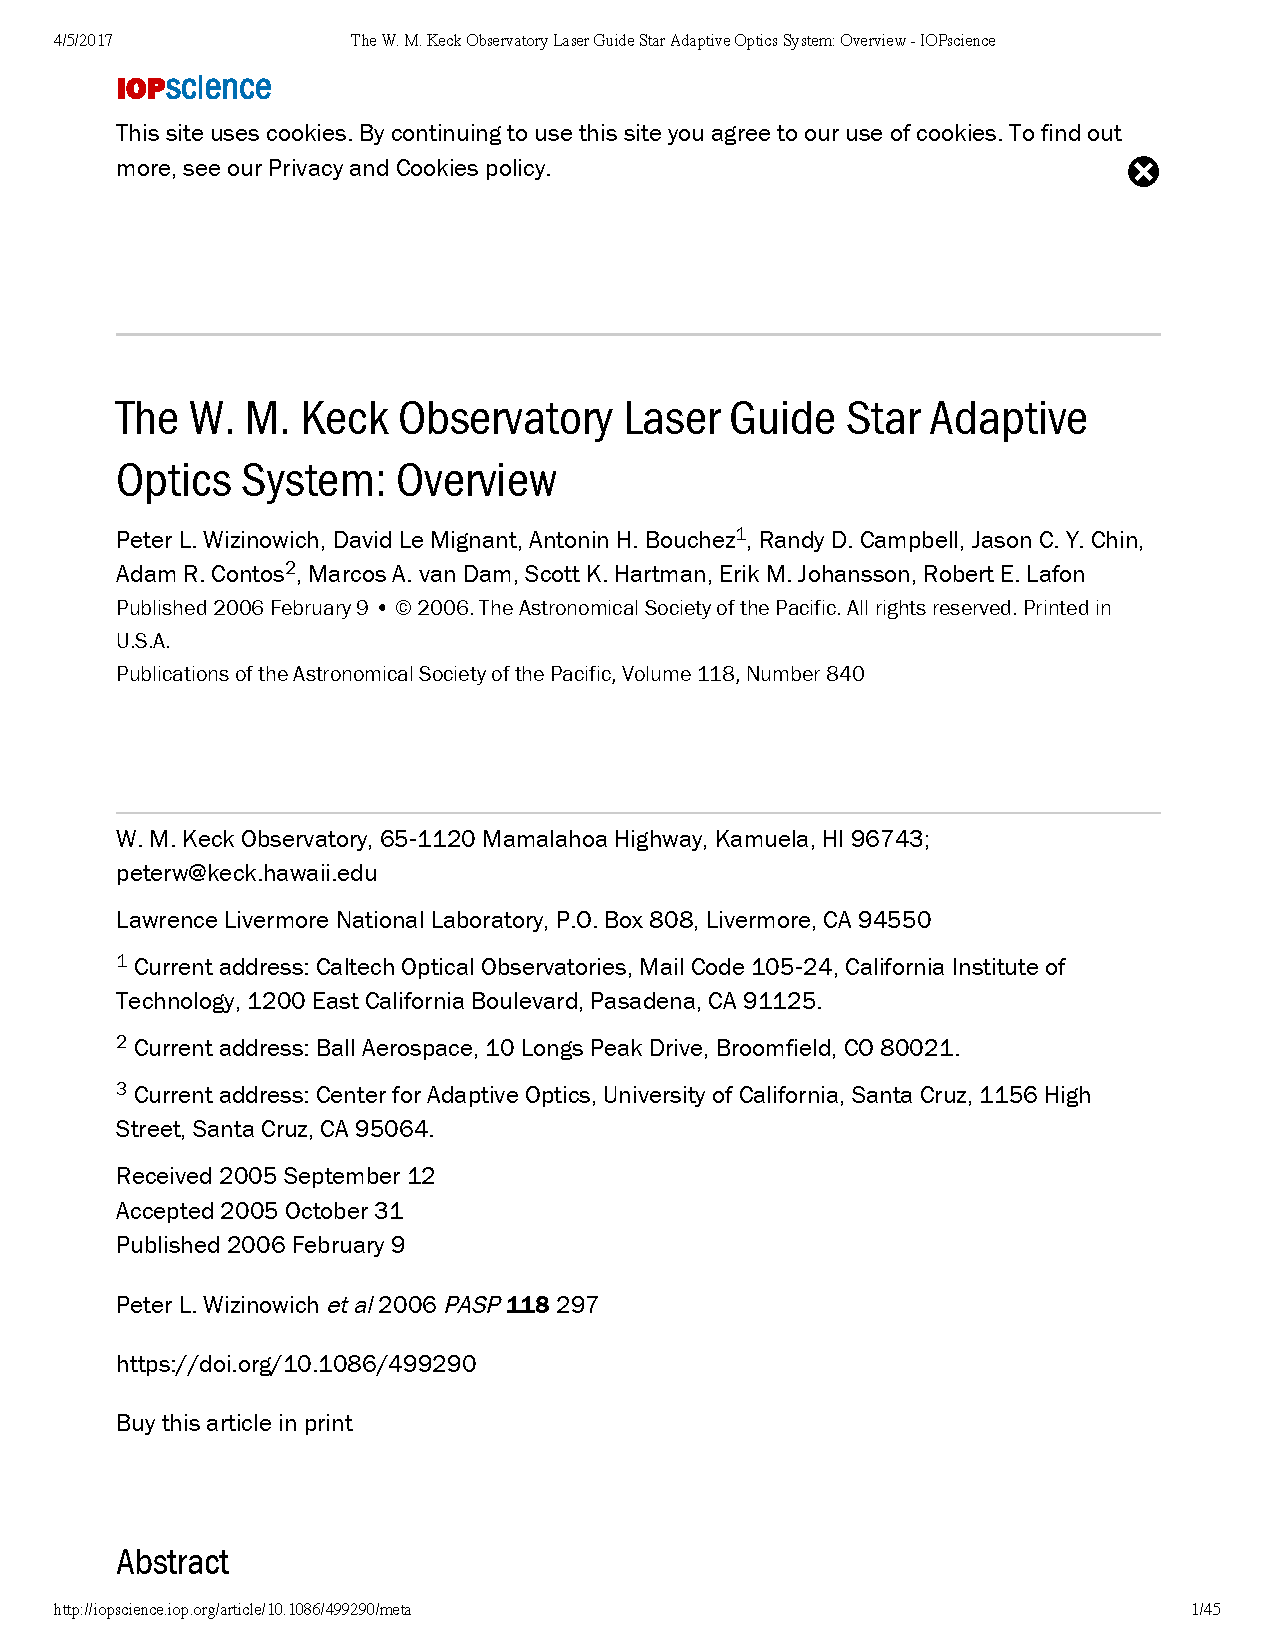
\includepdf[pages = 1-28]{PDF/Keck_observatory_system.pdf}

\pagebreak

\subsection{Continuously Tunable Picosecond Dye Laser}
\pagebreak
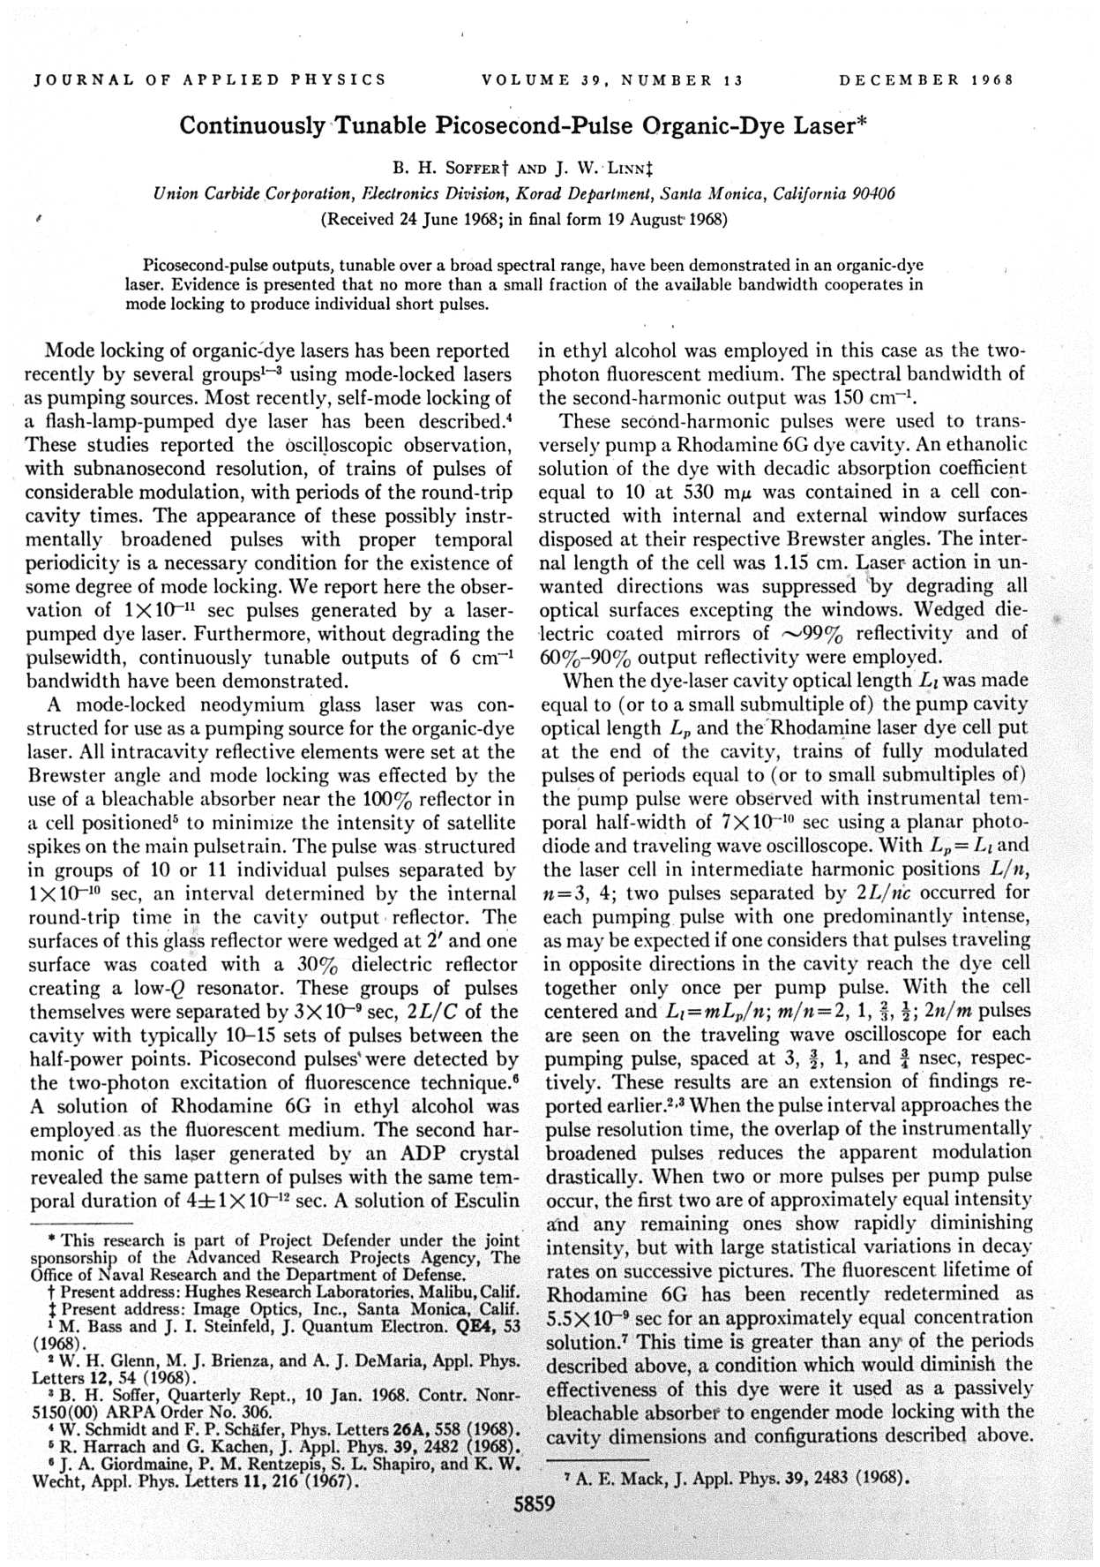
\includepdf[pages=-]{PDF/continuously_tunable_ps_dyelaser.pdf}
\pagebreak


\section{Citations}
\subsection{Brackman, LambdaChrome}
Brackman, Ulrick, “Lambdachrome Laser Dyes,” Lambda Physik 3, 2000
\subsection{Budker, Optical Magnetometry}
Budker, Dmitry, and Romalis, Michael. “Optical Magnetometry.” Nature Physics 3, 2007.
\subsection{Fan, Improving LGS through Polarization Switching}
Fan, Tingwei, Tianhua Zhou, and Yan Feng. "Improving sodium laser guide star brightness by polarization switching." Scientific reports 6 (2016).
\subsection{Fugate, Measuring Wavefront Distortion}
Fugate, Robert Q., and D. L. Fried. "Measurement of atmospheric wavefront distortion using scattered light from a laser guide-star." Nature 353.6340 (1991): 144.
\subsection{Gale, Kilohertz Picosecond Dye Laser}
Gale, G. M., B. Pedersen, and P. Schanne. "Kilohertz picosecond distributed-feedback dye laser system." Optics Communications 76.2 (1990): 138-142.
\subsection{Kane, Pulsed Laser Architecture}
Kane, Thomas J., Paul D. Hillman, and Craig A. Denman. "Pulsed laser architecture for enhancing backscatter from sodium." SPIE Astronomical Telescopes+ Instrumentation. International Society for Optics and Photonics, 2014.
\subsection{Kibblewhite, Physics of LGS}
Kibblewhite, Edward. "The physics of the sodium laser guide star: Predicting and enhancing the photon returns." In Advanced Maui Optical and Space Surveilance Technologies Conference. 2009.
\subsection{Rampy, Toward Optimization of pulsed LGS}
Rampy, Rachel, Donald Gavel, Simon M. Rochester, and Ronald Holzlöhner. "Toward optimization of pulsed sodium laser guide stars." JOSA B 32, no. 12 (2015): 2425-2434.
\subsection{Holzlohner, Optimization of CW LGS}
Holzlöhner, R., et al. "Optimization of cw sodium laser guide star efficiency." Astronomy \& Astrophysics 510 (2010): A20.
\subsection{Sohl (AJP), Modular Reconfigurable Pulsed Dye Laser}
Sohl, John E., and Stephen G. Payton. "A modular, reconfigurable-cavity, pulsed dye laser for the advanced undergraduate laboratory." American Journal of Physics 65.7 (1997): 640-652.
\subsection{Watanable, Advancement in Adaptive Optics}
Watanabe, Makoto, et al. "Proceedings of SPIE-The International Society for Optical Engineering." Advancements in Adaptive Optics. 2004.
\subsection{Wizinowich, W.M. Keck Observatory System}
Wizinowich, Peter L., David Le Mignant, Antonin H. Bouchez, Randy D. Campbell, Jason CY Chin, Adam R. Contos, Marcos A. van Dam et al. "The WM Keck Observatory laser guide star adaptive optics system: overview." Publications of the Astronomical Society of the Pacific 118, no. 840 (2006): 297.











\end{document}

